\documentclass[10pt]{article}
\usepackage[margin=0.8in]{geometry}
\usepackage{booktabs,pgfplots}
\pgfplotsset{compat=1.18}
\title{N12: Frozen held-out paired wall comparison}
\author{Reproducibility packet}
\date{25 October 2026}
\begin{document}
\maketitle
\noindent\textbf{Observed status.} No valid isolated 12-process schedule; 0/5,040 timed target-arm rows. The A/A rho-process ratio is null. Candidate/rho round median is null and minimum is null. No ratio is emitted unless all 5,040 target-arm rows and the isolation receipt pass. The independent-host operation-count ratio 2.4799052224835276 is separate.
\begin{center}
\begin{tabular}{rr}\toprule Paired round & candidate/rho process wall ratio \\ \midrule
1--5 & null \\
\bottomrule\end{tabular}
\end{center}
\begin{center}
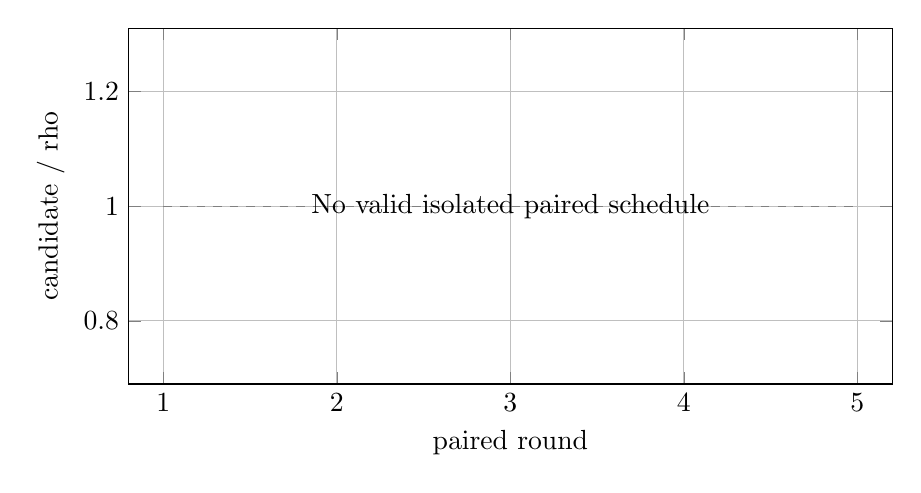
\begin{tikzpicture}
\begin{axis}[width=0.93\linewidth,height=6.1cm,xmin=0.8,xmax=5.2,ymin=0.6900,ymax=1.3100,xlabel={paired round},ylabel={candidate / rho},xtick={1,2,3,4,5},grid=major]
\addplot[dashed,gray] coordinates {(1,1)(5,1)};
\node at (axis cs:3,1) {No valid isolated paired schedule};
\end{axis}
\end{tikzpicture}
\end{center}
\noindent The frozen selector and 420 target IDs, source SHA-256 hashes, host manifest, schedule, and null rules are in the adjacent protocol and data dictionary. At the 09:03 UTC start gate the benchmark lock remained occupied, so the wall ratio is null. The adjacent obstruction note gives the exact lock and pressure observations. This PDF reports observed wall data only; it does not pool wall time with operation-count prices.
\end{document}
